\chapter{Simulations (10 pgs)}

This part of thesis serves as a widen documentation for the \texttt{PyVort} codebase, a new platform to simulate quantum vortex rings. The code is written in well commented Python 3, arranged in a modular structure. The primary aim of this documentation is to highlight which module(s) are involved and how they work.
In appendix, one can find a table of the parameters (user's options) which can be set in the \texttt{config.py} file.

To run the code, there has to be installed only Python 3 (with various libraries) on any OS. All the Python code can be found in the directory \texttt{src/}. The entire project is open-source and can be found as a public \href{https://github.com/KuboBahyl/superfluid}{GitHub} repository. Pull requests of any further development would be definitely appreciated.

At present, we use infinite boundary conditions. Therefore, only closed-loop vortices can be realized using simulation. However, the codebase is flexible and supports the potential implementation of unclosed loops.

\section{Vortex filament model}

The \texttt{PyVort} code is based on vortex filament (VF) model, a technique pioneerd by Schwarz in the early 1980s. Superfluid vortex filament is represented by a series of mesh points (segments) distributed along the centerline of the VF. The motion of the whole VF is summed up by the motion of each mesh point.

\begin{figure}[h]
	\centering
	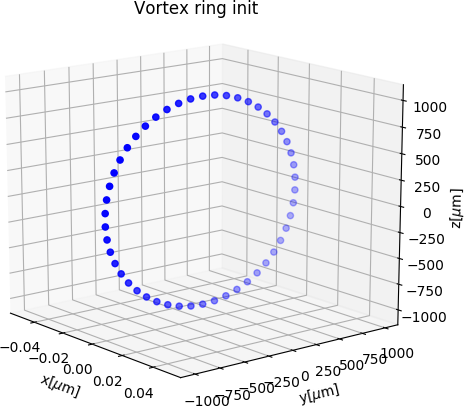
\includegraphics[width=0.5\textwidth]{graphics/simul/ring_init_crop}
	\caption{Example of vortex ring segments}
\end{figure}

As introduced in Theoretical Background, we define the VF more precisely as a three dimensional curve $\vec{s}(\xi, t)$. Here, $\xi$ represent an arc-lengths and $t$ is time. Each segment is given by its coordinates $\vec{s}_i$, direct neighbour indices (previous $(i-1)$ and next $(i+1)$). This resolves in a directed digraph of segments, which is a good starting point for the initial data structure.

Next we define the tangent vector $\vec{s}^{\prime}$, then normal vector $\vec{s}^{\prime\prime}$, and the binormal vector $\vec{s}^{\prime} \times \vec{s}^{\prime\prime}$ by taking numerical derivatives. Note $\vec{s}^{\prime} = \text{d}\vec{s} / \text{d}\xi$,
and so on. Numerical derivatives are achieved using Finite Differences method, as introduced in next subsection.


\subsection*{Finite differences}

In order to properly calculate the numerical derivatives $\vec{s}^{\prime}$ and $\vec{s}^{\prime\prime}$, belonging to the directed curve in 3D, we need to use a sophisticated numerical method. At a particular segment with position $\vec{s}_i$ , we define the distance to the particle in-front $\vec{s}_{i+1}$ as $l_{i} = \vert \vec{s}_i - \vec{s}_{i+1} \vert$ and the distance to the particle behind
$\vec{s}_{i-1}$ as $l_{i-1} = \vert \vec{s}_{i-1} - \vec{s}_i \vert$.
By in-front/behind we refer to the particles next/previous along the filament. Similarly, we can define the $l_{i+1}$ and $l_{i-2}$ for the farther segment lines.

\begin{figure}[h]
	\centering
	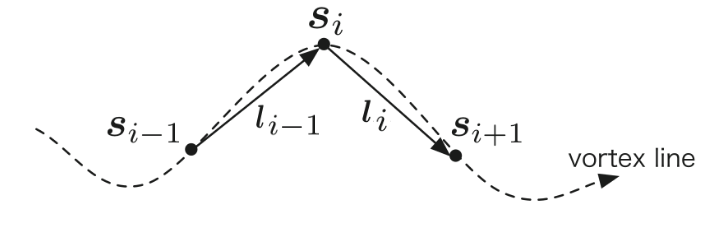
\includegraphics[width=0.8\textwidth]{graphics/simul/finite-diff}
	\caption{Depiction of a few segments and corresponding lengths}
\end{figure}

For accuracy, we approximate all the spatial derivatives $\vec{s}_i^{\prime}$, $\vec{s}_i^{\prime\prime}$ by a
fourth-order finite difference method (FD), which can also account the
varying distances along the vortex filament. With this, the first and second derivatives can be obtained based on coordinates of 2 closest neigbours (on each side).

Using FD theorem, we can construct the approximations by taking the Taylor's series expansions. We can then write:

\begin{equation}
\frac{\text{d}^n\vec{s}_i}{\text{d}\xi^n} \approx
A_i\vec{s}_{i-2} +
B_i\vec{s}_{i-1} +
C_i\vec{s}_{i} +
D_i\vec{s}_{i+1} +
E_i\vec{s}_{i+2}
\hspace{1cm}
\text{for} \,n\in\{1,2\}
\end{equation}

Calculation of coefficients $A, B, C, D, E$ can be done in many ways. In code, we use both the analytical solution (closed form) and the solution by inverting the Vandermonde matrix. The first one is obviously faster, but the second one is scalable. By \textit{scalability}, we mean that if we would decide to calculate derivatives based on nearest $n>4$ neighbours, the Vandermonde method can be still used, whereas the closed-form solutions won't be more available. However, the inverting process of Vandermonde matrix is computationally expensive and doesn't have to converge sometimes.

In this work, we used the closed-form solution (4 neighbours) and left the Vandermonde method as an \texttt{except} case for the higher-level mode.

\subsection*{Biot-Savart discretisation}

We denote the static external sources of velocity fields (which can be set in \texttt{config.py}) as $\vec{v}_{n,ext}$ and $\vec{v}_{s,ext}$. The equation of motion for given segment is then given directly by Schwarz's equation(\ref{schwarz}):

\begin{equation}
\frac{\text{d}\vec{s}_i}{\text{d}t} =
\vec{v}_{s,ext} + \vec{v}_{\text{ind}}^{(i)} + \vec{v}_{\text{drive}}^{(i)}
\end{equation}

The first difficulty in the VF model comes from the calculation of term $\vec{v}_{\text{ind}}$. As we shown previously (\ref{lia+biot}), this advection term can be split into the LIA part and a Biot-Savart integral:

\begin{equation}
\vec{v}_{\text{ind}}^{(i)} =
\vec{v}_{\text{LIA}}^{(i)} + \vec{v}_{\text{BIOT}}^{(i)} =
\frac{\varkappa}{4\pi} (\vec{s}^{\prime}_i \times \vec{s}^{\prime \prime}_i)
\ln{\Bigg(\frac{2\sqrt{l_{i-1} l_i}}{a}\Bigg)}
+ \frac{\varkappa}{4\pi} \int_{\mathcal{L}^{\prime}} \frac{(\vec{r^{\prime}} - \vec{s}_i) \times \text{d}\vec{r^{\prime}}}{\vert \vec{r^{\prime}} - \vec{s}_i \vert^3}\,,
\end{equation}

where $l_{i-1}$ and $l_i$ are the arc lengths of the curve between
points $\vec{s}_{i-1}$ and $\vec{s}_i$ and between $\vec{s}_i$ and $\vec{s}_{i+1}$ respectively, and $\mathcal{L}^{\prime}$ is the original vortex line without the two segment lines between $\vec{s}_{i-1}$ and $\vec{s}_{i+1}$.

Using the segment discretisation, the Biot-Savart integral can be rewritten into the sum of single-line contributions between each $j$-th and $j+1$-th segment (except for the ones attached to the $i$-th point):

\begin{equation}
\vec{v}_{\text{BIOT}}^{(i)} \approx
\frac{\varkappa}{4\pi}
\sum_{j \notin \{i-1, i\}}
\frac{(R_j + R_{j+1}) (\vec{R}_j \times \vec{R}_{j+1})}{R_j R_{j+1} (R_j R_{j+1} + \vec{R}_j \dotprod \vec{R}_{j+1})}\,,
\end{equation}

where $\vec{R}_j = \vec{s}_j - \vec{s}_i$ and $\vec{R}_{j+1} = \vec{s}_{j+1} - \vec{s}_i$ are the relative vectors from the given point.

\begin{figure}[h]
	\centering
	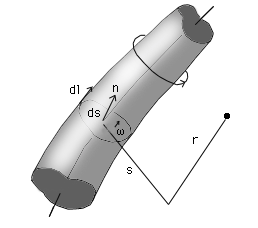
\includegraphics[width=0.5\textwidth]{graphics/simul/biot}
	\caption{The infinitesimal contribution of a segment line between two points $\vec{s}_j$ and $\vec{s}_{j+1}$ at a given point $\vec{r}$.}
\end{figure}

Note that, if one takes in account the Biot-Savart law for $N$ mesh points, the computational time is proportional to $\mathcal{O}(N^2)$, while, if one uses just the LIA term, it is only $\mathcal{O}(N)$. Numerical simulations based on Biot-Savart are therefore far expensive and not practical, even with the speed of today's computers.

One way to get around this difficulty is to update the LIA term. In this method we neglect completely the non-local Biot-Savart integral and keep just the local term. This is typically done with a minor adjustments within the log term:

\begin{equation}
\vec{v}_{\text{LIA}}^{(i)} =
\frac{\varkappa}{4\pi} (\vec{s}^{\prime}_i \times \vec{s}^{\prime \prime}_i)
\ln{\Bigg(\frac{2 R_i}{a}\Bigg)}\,,
\end{equation}

where $R_i$ is a filament length scale - may be taken as a local curvature of $i-th$ segment: $R_i = 1 / \vert \vec{s}^{\prime \prime}_i \vert$. Updated LIA is a very convenient approximation and works very well for calculating the motion of a single vortex ring.

\subsection*{State definition}

In code, a single vortex ring object is represented using the \texttt{class} structure. This structure is partially updated after each time step and works as a source of truth. We will call it as the \textit{state} of the vortex ring and it is defined (and initialised) with following properties:

\begin{itemize}
	\item \underline{shape} - a dictionary of three parameters: ring center coordinates $[x_c,y_c,z_c]$, radius $R$ and the direction of desired motion $\{x, y, z\}$ (three possible axis)
	\item \underline{velocity} - the actual velocity magnitude of vortex ring center $\vert \vec{v}_c \vert$
	\item \underline{number of segments} - number of segments $N$ the vortex ring is composed of
	\item \underline{segments} - an array of all segments, each one with following attributes:
	\begin{itemize}
		\item \underline{coordinates} - an array of segment coordinates $\vec{s}_i = [x_i,y_i,z_i]$
		\item \underline{previous/next neighbour} - array localisation indices of the \textit{previous} $(i-1)$ and the \textit{next} $(i+1)$ segment within the context of the directed vortex
		\item \underline{tangent/curvature} - a tangential and normal vectors $\vec{s}^{\prime}_i$ and $\vec{s}^{\prime\prime}_i$

		\item \underline{LIA velocity} - a self-induced velocity $\vec{v}_{\text{LIA}}^{(i)}$ driven by the local curvature.
		\item \underline{BIOT velocity} - a self-induced velocity driven by the farther segment lines of the vortex ring $\vec{v}_{\text{BIOT}}^{(i)}$

		\item \underline{Drive velocity} - a velocity given by the mutual friction force $\vec{v}_{\text{drive}}^{(i)}$
		\item \underline{Full velocity} - the sum of external sources $\vec{v}_{s,ext}$, LIA velocity $\vec{v}_{\text{LIA}}^{(i)}$, BIOT velocity $\vec{v}_{\text{BIOT}}^{(i)}$ and the drive velocity $\vec{v}_{\text{drive}}^{(i)}$, resulting in $\text{d}\vec{s}_i / \text{d}t$
	\end{itemize}
\end{itemize}

The proper initialisation of the \textit{state} in the very beginning of simulation includes the following steps:
\begin{itemize}
	\item[1.] an input from user: \textit{center, radius} and \textit{direction}
	\item[2.] the gradual initialisation of neigbour indices (to an $i$-th element in segment array will be assigned $i-1$ index as the \textit{previous} and $i+1$ index as the \textit{next} neighbour index )
	\item[3.] Calculation of all $\vec{s}^{\prime}$ and $\vec{s}^{\prime\prime}$ using Finite differences method
	\item[4.] Calculation of all segment velocities using motion equations and their approximative forms
	\item[5.] Calculation of the center velocity by taking the mean of all segments' full velocites in corresponding direction
\end{itemize}

\newpage

\section{Time evolution}

Now when we defined and ran all the necessary calculations leading to the quantum vortex ring's \textit{state} fulfillment, we can start to propagate it in time.

\begin{figure}[h]
	\centering
	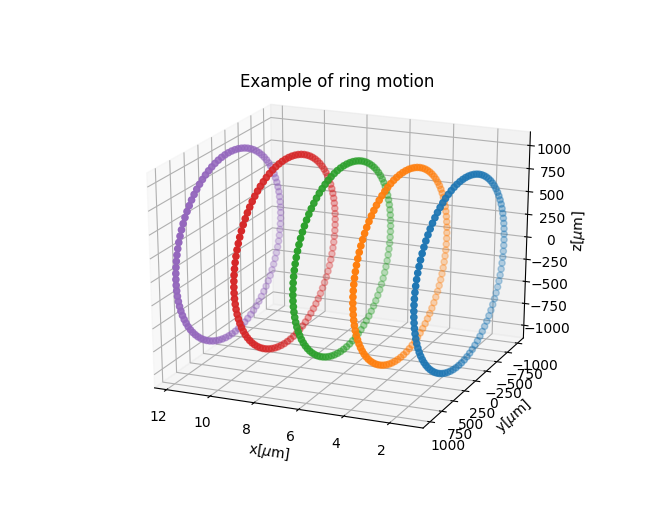
\includegraphics[width=0.8\textwidth]{graphics/simul/time-example}
	\caption{Example of a moving vortex ring}
\end{figure}

\subsection*{Time stepping}

Time evolution is based on an explicit iterative method: the fourth-order Runge-Kutta (RK4) scheme. When we consider the Schwarz's equation $\text{d}\vec{s}_i / \text{d}t \equiv \vec{v}_{\text{full}}^{(i)}$, the stepping algorithm is given as:

\begin{equation}
\vec{s}_{i}(t+\text{d}t) =
\vec{s}_{i}(t) +
\frac{\text{d}t}{6} (\vec{v}_1^{(i)} + 2\vec{v}_2^{(i)} + 2\vec{v}_3^{(i)} + \vec{v}_4^{(i)})\,,
\end{equation}

where $\text{d}t$ is the time step and the velocities $\vec{v}_1^{(i)}, \vec{v}_2^{(i)}, \vec{v}_3^{(i)}, \vec{v}_4^{(i)}$ are the induced velocites of partial steps:

\begin{align}
\vec{v}_1^{(i)} =& \vec{v}_{\text{full}}^{(i)}
(\vec{s}_i, t)\,,
\\
\vec{v}_2^{(i)} =& \vec{v}_{\text{full}}^{(i)}
(\vec{s}_i + \vec{v}_1^{(i)} \text{d}t / 2, t + \text{d}t / 2)\,,
\\
\vec{v}_3^{(i)} =& \vec{v}_{\text{full}}^{(i)}
(\vec{s}_i + \vec{v}_2^{(i)} \text{d}t / 2, t + \text{d}t / 2)\,,
\\
\vec{v}_4^{(i)} =& \vec{v}_{\text{full}}^{(i)}
(\vec{s}_i + \vec{v}_3^{(i)} \text{d}t, t + \text{d}t)
\end{align}

Lower-order schemes such as basic Euler method is also implemented in code, however, not recommended to use. More on this is discussed in Results part of thesis.

The time step $\text{d}t$ is chosen so that the vortex ring cannot move faster than a $1\%$ of its size in a single step. As we will see later in Results, in case of vortex rings with changing radius, the time step $\text{d}t$ has to be iteratively changing after each break of the above rule:

\begin{equation}
\text{d}t \leftarrow \frac{0.01 R}{\vert \vec{v}_c \vert}
\end{equation}

\section{Re-segmentation of vortex}

Since the CPU time cost of a vortex simulation rises rapidly as the number of segments $N$ increases, it is importnant to manage this number so that the simulation can run as fast as possible. As the distance between neighbouring segments is compressed/enlarged with time, there is need to remove/add segments to conserve the mesh resolution. The closeness (in terms of arclength) of neighbouring segments has to be measured at each step and the criteria for \textit{re-segmentation} heavily depends on the simulation itself and a scale at which we desire to observe any phenomena.

The simplest re-segmenting criteria is to attempt to keep an approximately \textit{uniform distance} between the segments. To ensure  this, two important conditions were implemented:

\begin{itemize}
	\item[1.] The segment $\vec{s}_{j+1}$ would be removed if:

	\begin{equation}
	\vert \vec{s}_{j+1} - \vec{s}_j \vert < \delta_{\text{min}}\,,
	\end{equation}

	where $\delta_{\text{min}}$ is the minimal distance between two segments. Also, the segment $\vec{s}_j$ would take place somewhere between $\vec{s}_{j-1}$ and $\vec{s}_{j+2}$ so that it will conserve the curvature of vortex. Such result can be obtained using any spline interpolation along nearest neighbours. We worked with 3D local spline using 4 points (in our context they would be $\vec{s}_{j-2}$, $\vec{s}_{j-1}$, $\vec{s}_{j+1}$, $\vec{s}_{j+2}$) and create another 11 interpolated knots.
	Consequently, the new position of $\vec{s}_j$ will sit on the 6-th (the middle one) knot and also.

	\item[2.] In a similar manner, we add a new segment $\vec{s}_{\text{new}}$ between $\vec{s}_{j}$ and $\vec{s}_{j+1}$ if:

	\begin{equation}
	\vert \vec{s}_{j+1} - \vec{s}_j \vert > \delta_{\text{max}}\,,
	\end{equation}

	where $\delta_{\text{max}}$ is the maximal allowed distance between two segments.
\end{itemize}

This will keep all the distances along the vortex rougly in the range $\delta_{\text{min}}$ to $\delta_{\text{max}}$ and also will keep the geometrical properties. However, when adding/removing points from the segment array, one has to also shift the indices of all segments, which adds unnecessary complexity into the simulation.

\section{Future implementations}

To make \texttt{Pyvort} a full-fledged quantum vortex simulation, there should be implemented following improvements:

\subsection*{Complexity speedup}

Recent numerical research presented \cite{tree_alg} a new numerical method to compute the evolution of vortex filament. The method is based on a \textit{tree algorithm} which considerably speeds up the calculation of Biot-Savart integrals - computational cost scales as $\mathcal{O}(N \log(N))$ rather than $N^2$. Properties of the tree method was tested for a variety of vortex configurations, ranging from simple vortex rings to a counterflow vortex tangle and compared with the LIA approac and the exact Biot-Savart's law.

Implementation of such algorithm is not easy, but definitely worth to obtain higher precision.


\subsection*{Re-connection process}

If any two lines become very close (less than the minimal separation $\delta_{\text{min}}$ along the line) the filaments can reconnect, changing the topology of the system. Many researchers claim this can happen, from analogies with vortex dynamics in the Navier–Stokes equation. Also, numerical studies of Gross–Pitaevskii equation showed that quantized vortices can reconnect.

\begin{figure}[h]
	\centering
	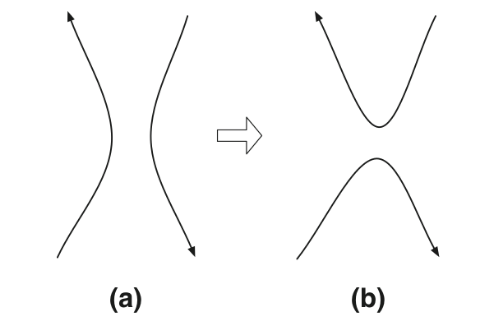
\includegraphics[width=0.6\textwidth]{graphics/simul/reconnection}
	\caption{Reconnection of quantized vortices. \textbf{(a)} Two vortices before reconnection, about to contact each other. \textbf{(b)} The new vortices after reconnection.}
\end{figure}

The VF model itself cannot describe the reconnection process because the vortex core structure is neglected. Hence, some artificial procedures must be introduced to simulate such process. For instance, when two vortices approach within a critical distance $\delta_{\text{min}}$, we will artificially reconnect the vortices.

The main criteria for reconnection is that the total length (this is corresponding with energy) will decrease. Self-reconnections (e.g. caused by a twist of vortex) would be treated in the same way. Since recconection ivolves only antiparallel vortices, one has to check using the inner product whether two vortices could physically reconnect or not.

\subsection*{High-order tests}

Once the code of interacting vortex filaments is developed, one has to face with the analysis of all that mass of data. The simplest measurable quantity is the total lenght of all vortex lines. In a finite volume this would be $L = (1/V) \int \text{d}\xi$ for the vortex line per unit volume.

Of course, there can be defined more complicated metrics, measuring the isotrophy of the vortex tangle. One of them is the length of line projected along a given vector $\vec{\hat{r}}$, give as:

\begin{equation}
J(\vec{\hat{r}}) = \frac{1}{VL} \int_{\mathcal{L}} \sqrt{1 - (\vec{s}^{\prime}(\xi) \dotprod \vec{\hat{r}})^2} \text{d}\xi
\end{equation}




\newpage
